\documentclass[aspectratio=169]{beamer}

\usepackage[utf8]{inputenc}
\usepackage[T1]{fontenc}
\usepackage{graphicx}
\usepackage{booktabs}
\usepackage{amsmath}

\usetheme{Madrid}
\setbeamertemplate{navigation symbols}{}

\title[Machine Vision Project]{From-Scratch CNN Classification, Pure-Noise GAN Augmentation, and CycleGAN Style Transfer}
\author[Qifeng LIU]{Qifeng LIU}
\date{}

\begin{document}

\begin{frame}
  \titlepage
\end{frame}

\begin{frame}{Dataset and Project Objective}
\small
\begin{itemize}
  \item Three tasks:
  \begin{itemize}
    \item Task 1: classify cows vs horses with a CNN trained from scratch
    \item Task 2: improve classification with GAN-based data augmentation
    \item Task 3: perform unpaired style transfer between the two classes
  \end{itemize}
  \item Dataset size:
  \begin{itemize}
    \item 82 training images and 82 test images
    \item 41 cows and 41 horses in each split
  \end{itemize}
  \item Main difficulty:
  \begin{itemize}
    \item one training instance per class
    \item unseen test instances
    \item shared viewpoint grid
  \end{itemize}
  \item Main objective:
  \begin{itemize}
    \item improve the weak horse class without making the classifier unstable
  \end{itemize}
\end{itemize}
\end{frame}

\begin{frame}{Task 1: CNN Design}
\footnotesize
\begin{columns}[T]
\column{0.54\textwidth}
\begin{itemize}
  \item Compact from-scratch CNN
  \begin{itemize}
    \item 3 blocks of \texttt{Conv + BN + ReLU + MaxPool}
    \item global average pooling
    \item small fully connected head: $64 \rightarrow 32 \rightarrow 2$
  \end{itemize}
  \item Why small?
  \begin{itemize}
    \item dataset is tiny
    \item overfitting is the main risk
  \end{itemize}
  \item Training choices
  \begin{itemize}
    \item class-weighted cross-entropy loss
    \item cow:horse weight ratio = $1:5$
    \item 3 fixed seeds
  \end{itemize}
  \item Final decision rule
  \begin{itemize}
    \item average logits across the 3 seed models
    \item then take the final class prediction
  \end{itemize}
\end{itemize}
\column{0.46\textwidth}
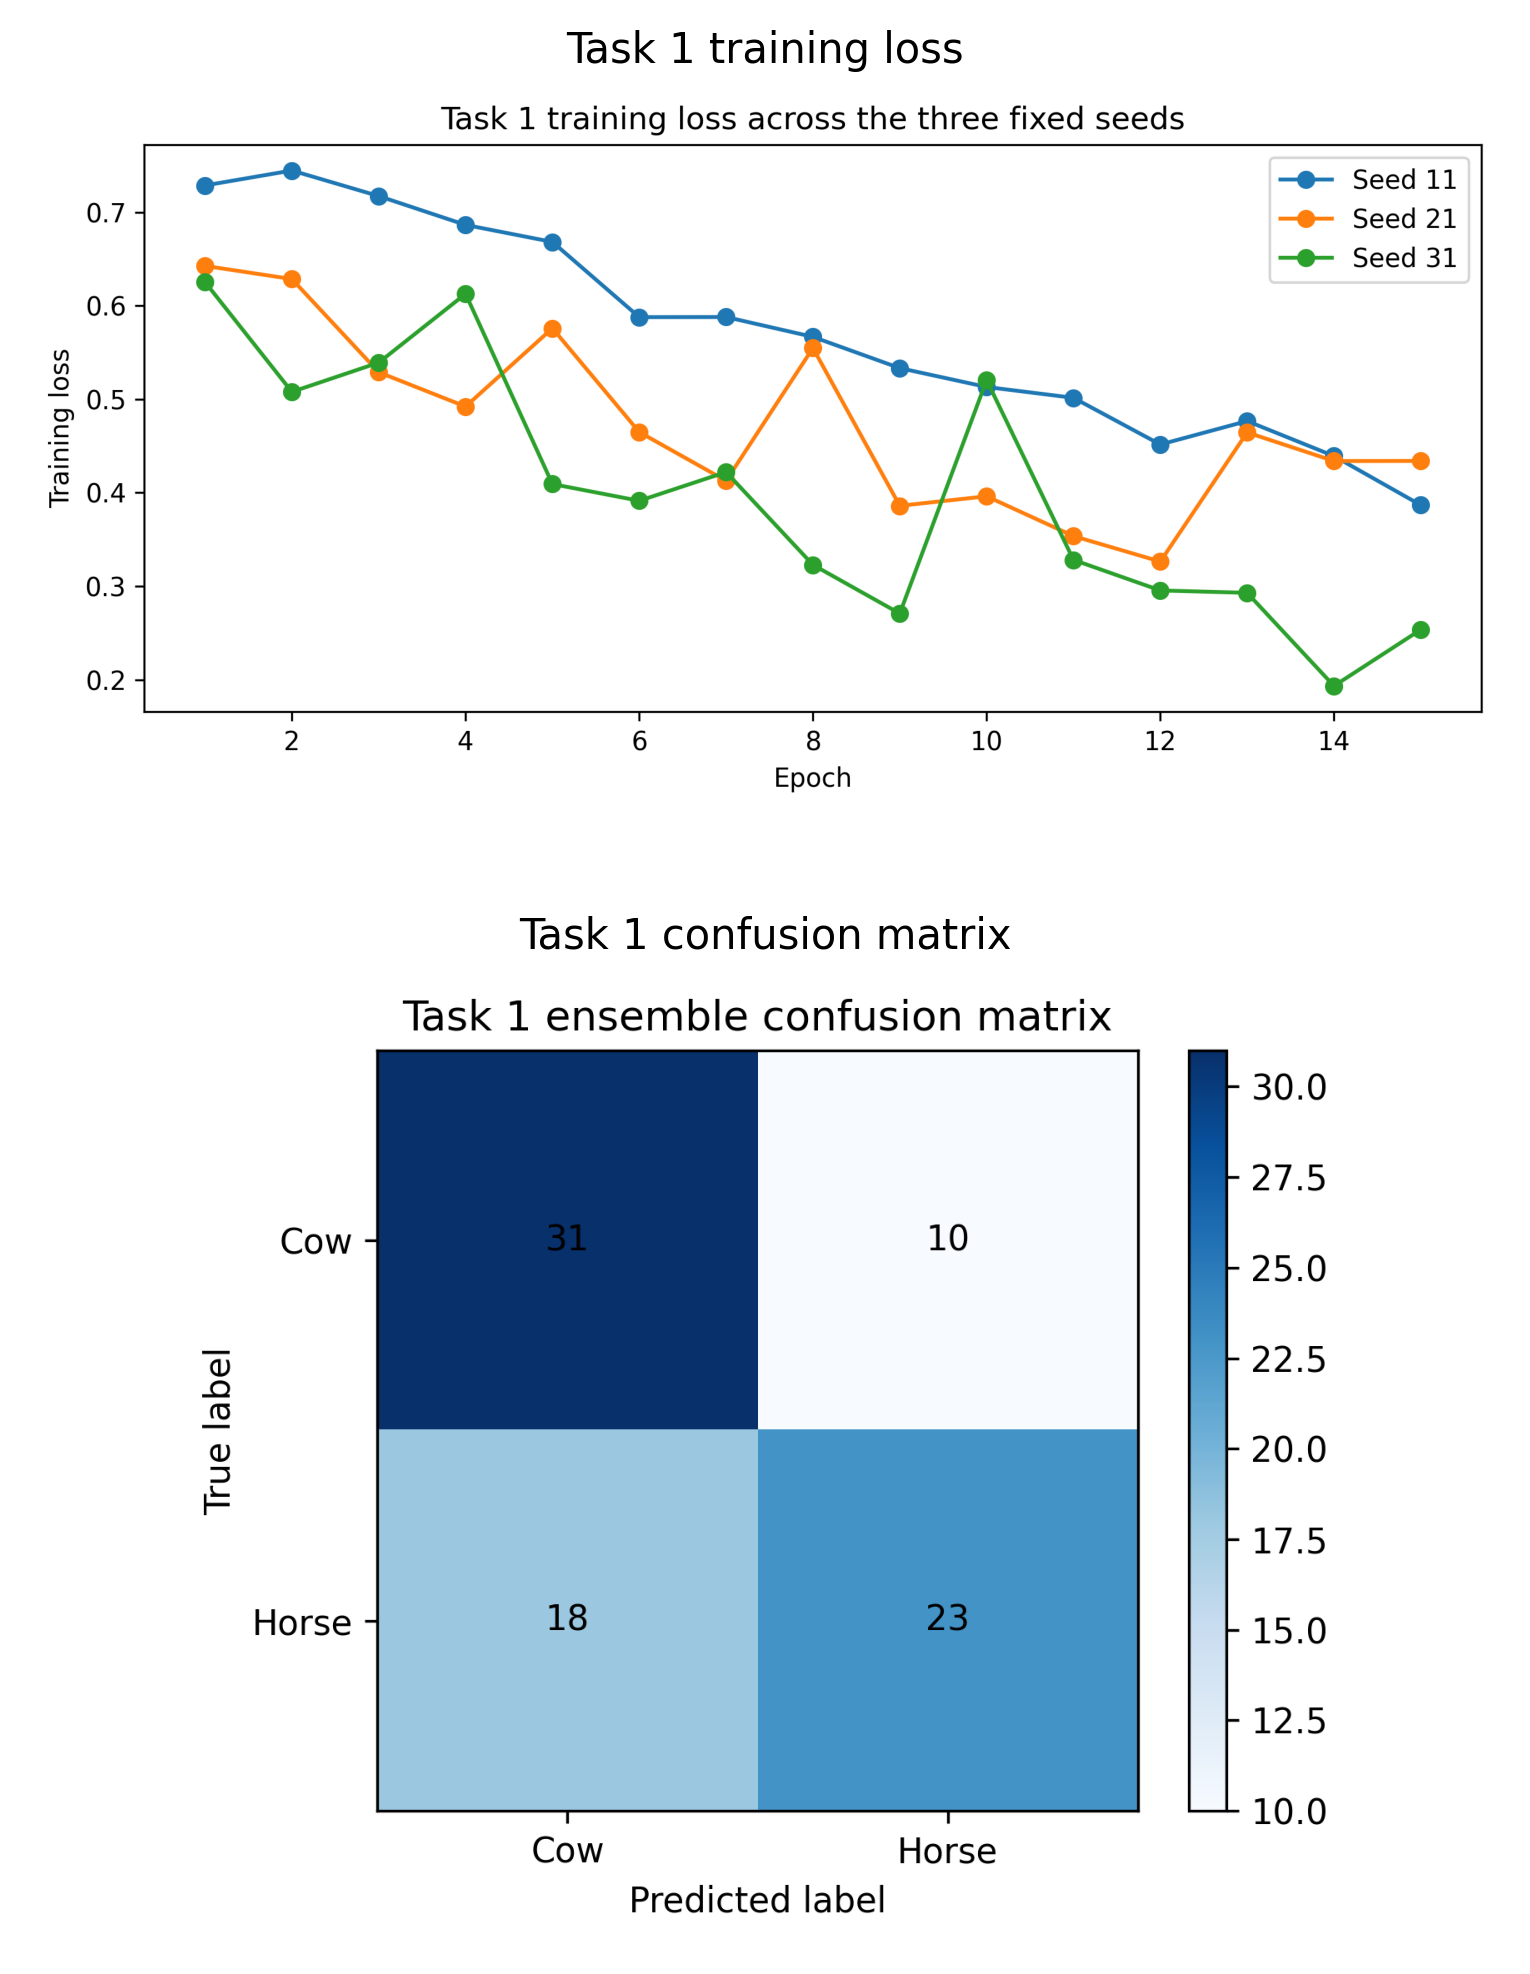
\includegraphics[width=\linewidth,height=0.69\textheight,keepaspectratio]{generated/figures/task1_overview.png}
\end{columns}
\end{frame}

\begin{frame}{Task 1: Results and Key Point}
\footnotesize
\begin{columns}[T]
\column{0.46\textwidth}
\begin{block}{Final Task 1 Ensemble}
\begin{tabular}{lr}
\toprule
Metric & Value \\
\midrule
Overall accuracy & 65.85\% \\
Cow accuracy & 75.61\% \\
Horse accuracy & 56.10\% \\
\bottomrule
\end{tabular}
\end{block}

\vspace{0.4em}
\begin{itemize}
  \item The CNN already works well from scratch.
  \item The most important stabilizers are:
  \begin{itemize}
    \item class-weighted cross-entropy loss
    \item cow:horse weight ratio = $1:5$
    \item logit-level ensemble
  \end{itemize}
  \item The remaining weakness is horse recognition.
\end{itemize}
\column{0.54\textwidth}
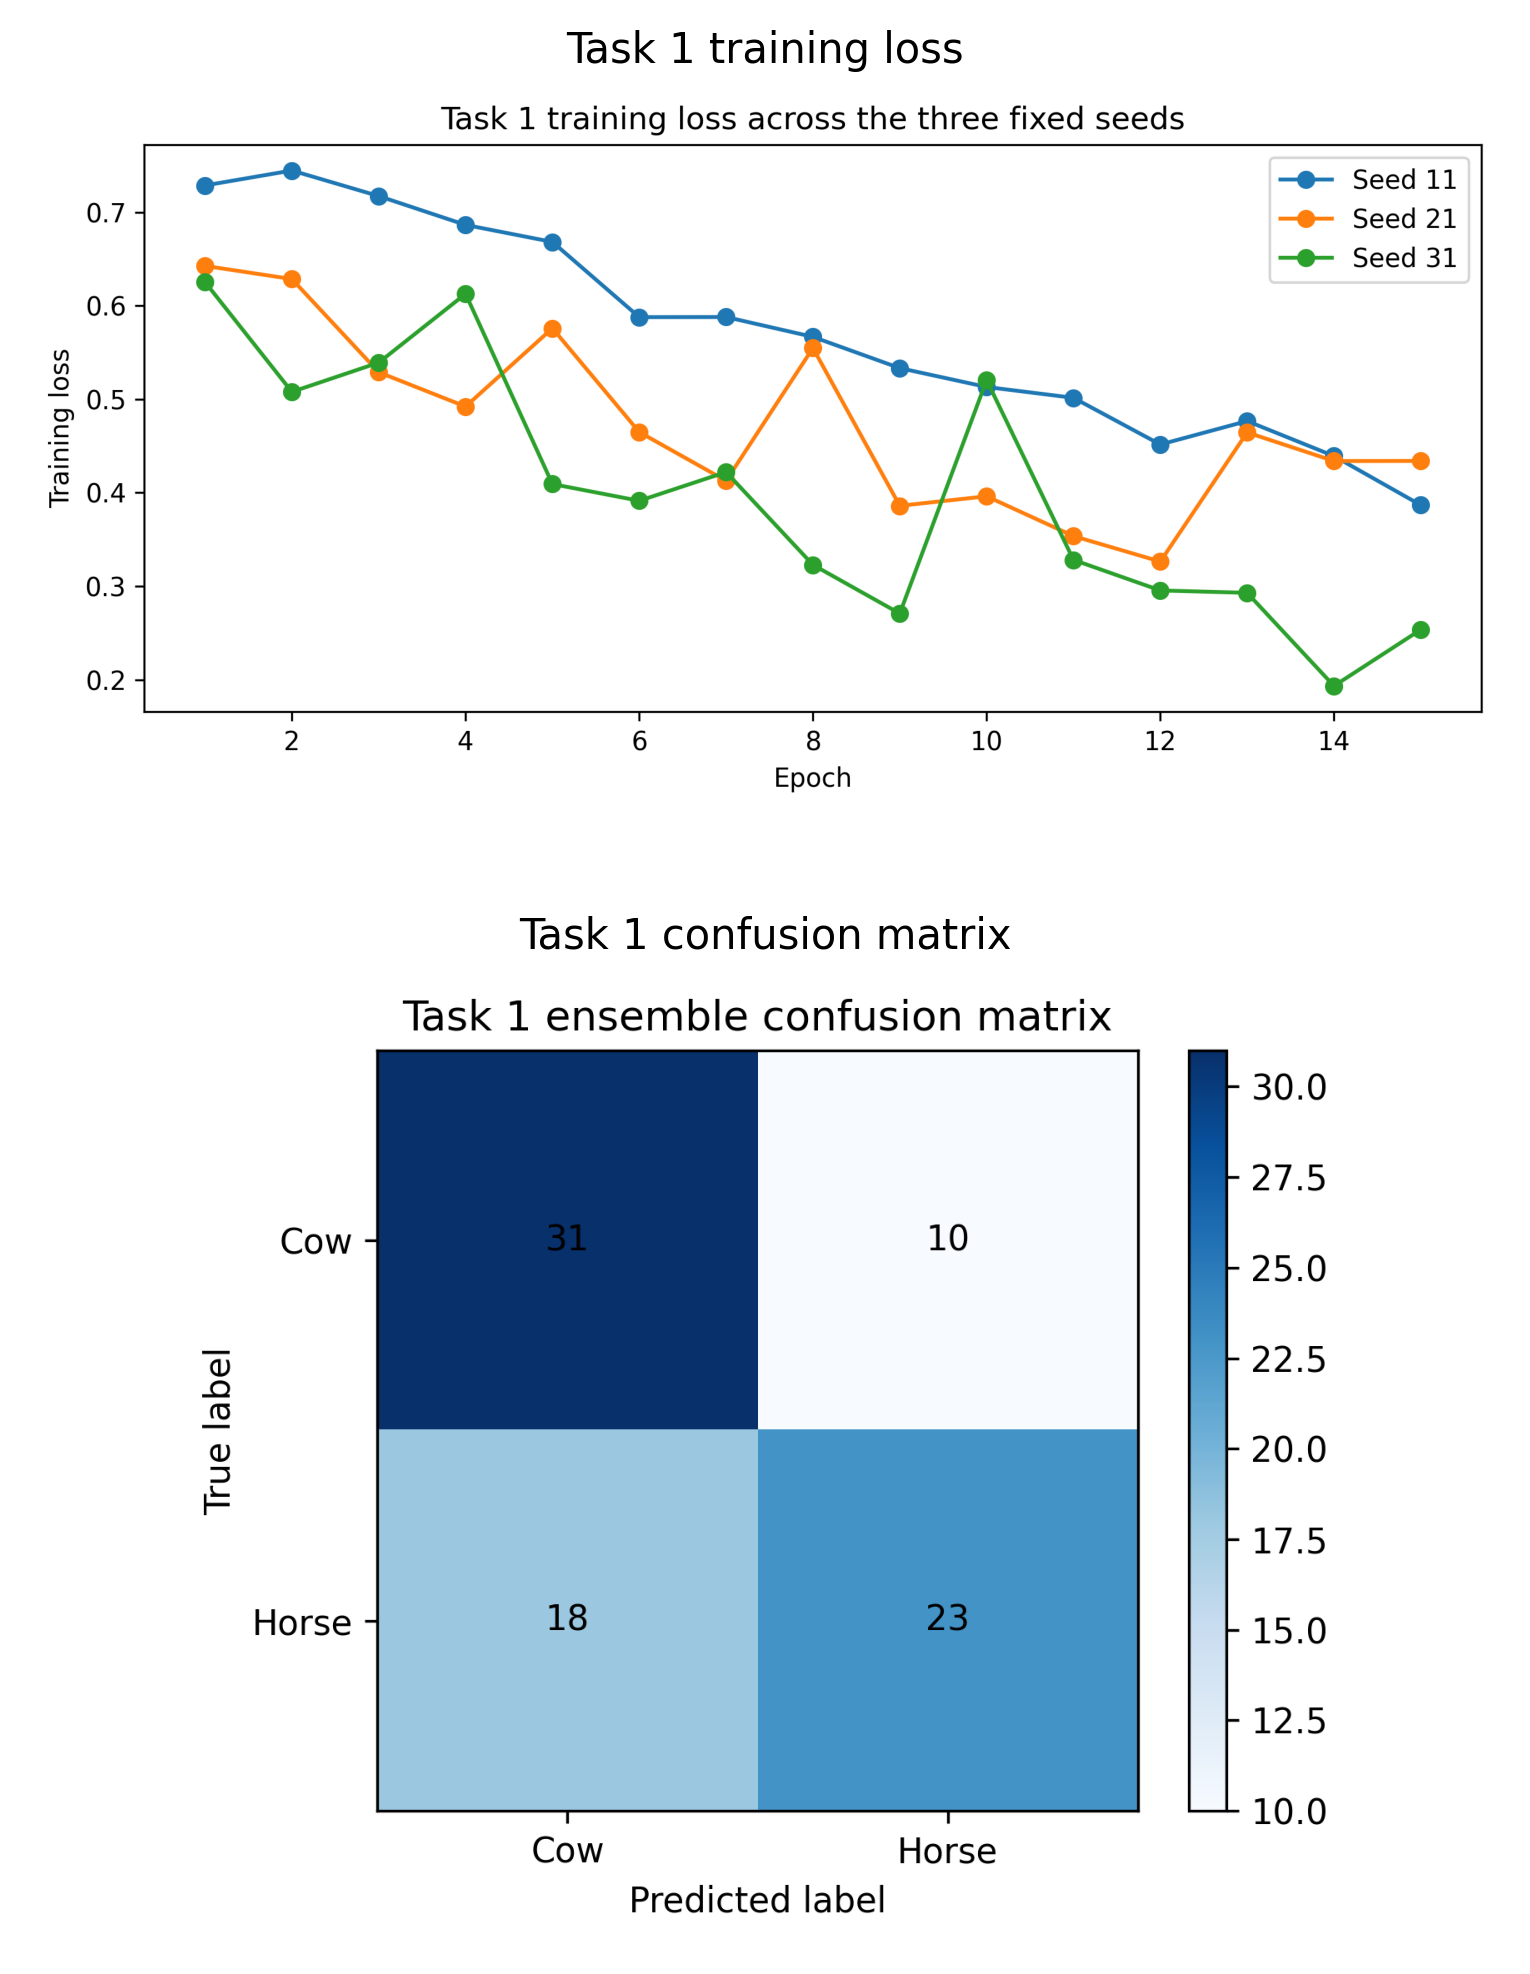
\includegraphics[width=\linewidth,height=0.72\textheight,keepaspectratio]{generated/figures/task1_overview.png}
\end{columns}
\end{frame}

\begin{frame}{Task 2: Pure-Noise GAN Architecture}
\footnotesize
\begin{columns}[T]
\column{0.46\textwidth}
\begin{itemize}
  \item Generator
  \begin{itemize}
    \item input latent vector $z \in \mathbb{R}^{100}$
    \item projection to feature map, then progressive \texttt{Upsample + Conv2d}
    \item \texttt{BatchNorm + LeakyReLU}, final \texttt{Tanh}
  \end{itemize}
  \item Discriminator
  \begin{itemize}
    \item stride-2 convolution blocks
    \item \texttt{LeakyReLU} and dropout
    \item binary real/fake prediction
  \end{itemize}
  \item Class-specific training
  \begin{itemize}
    \item one GAN for cows
    \item one GAN for horses
    \item valid generated images are exported for manual selection
  \end{itemize}
\end{itemize}
\column{0.54\textwidth}
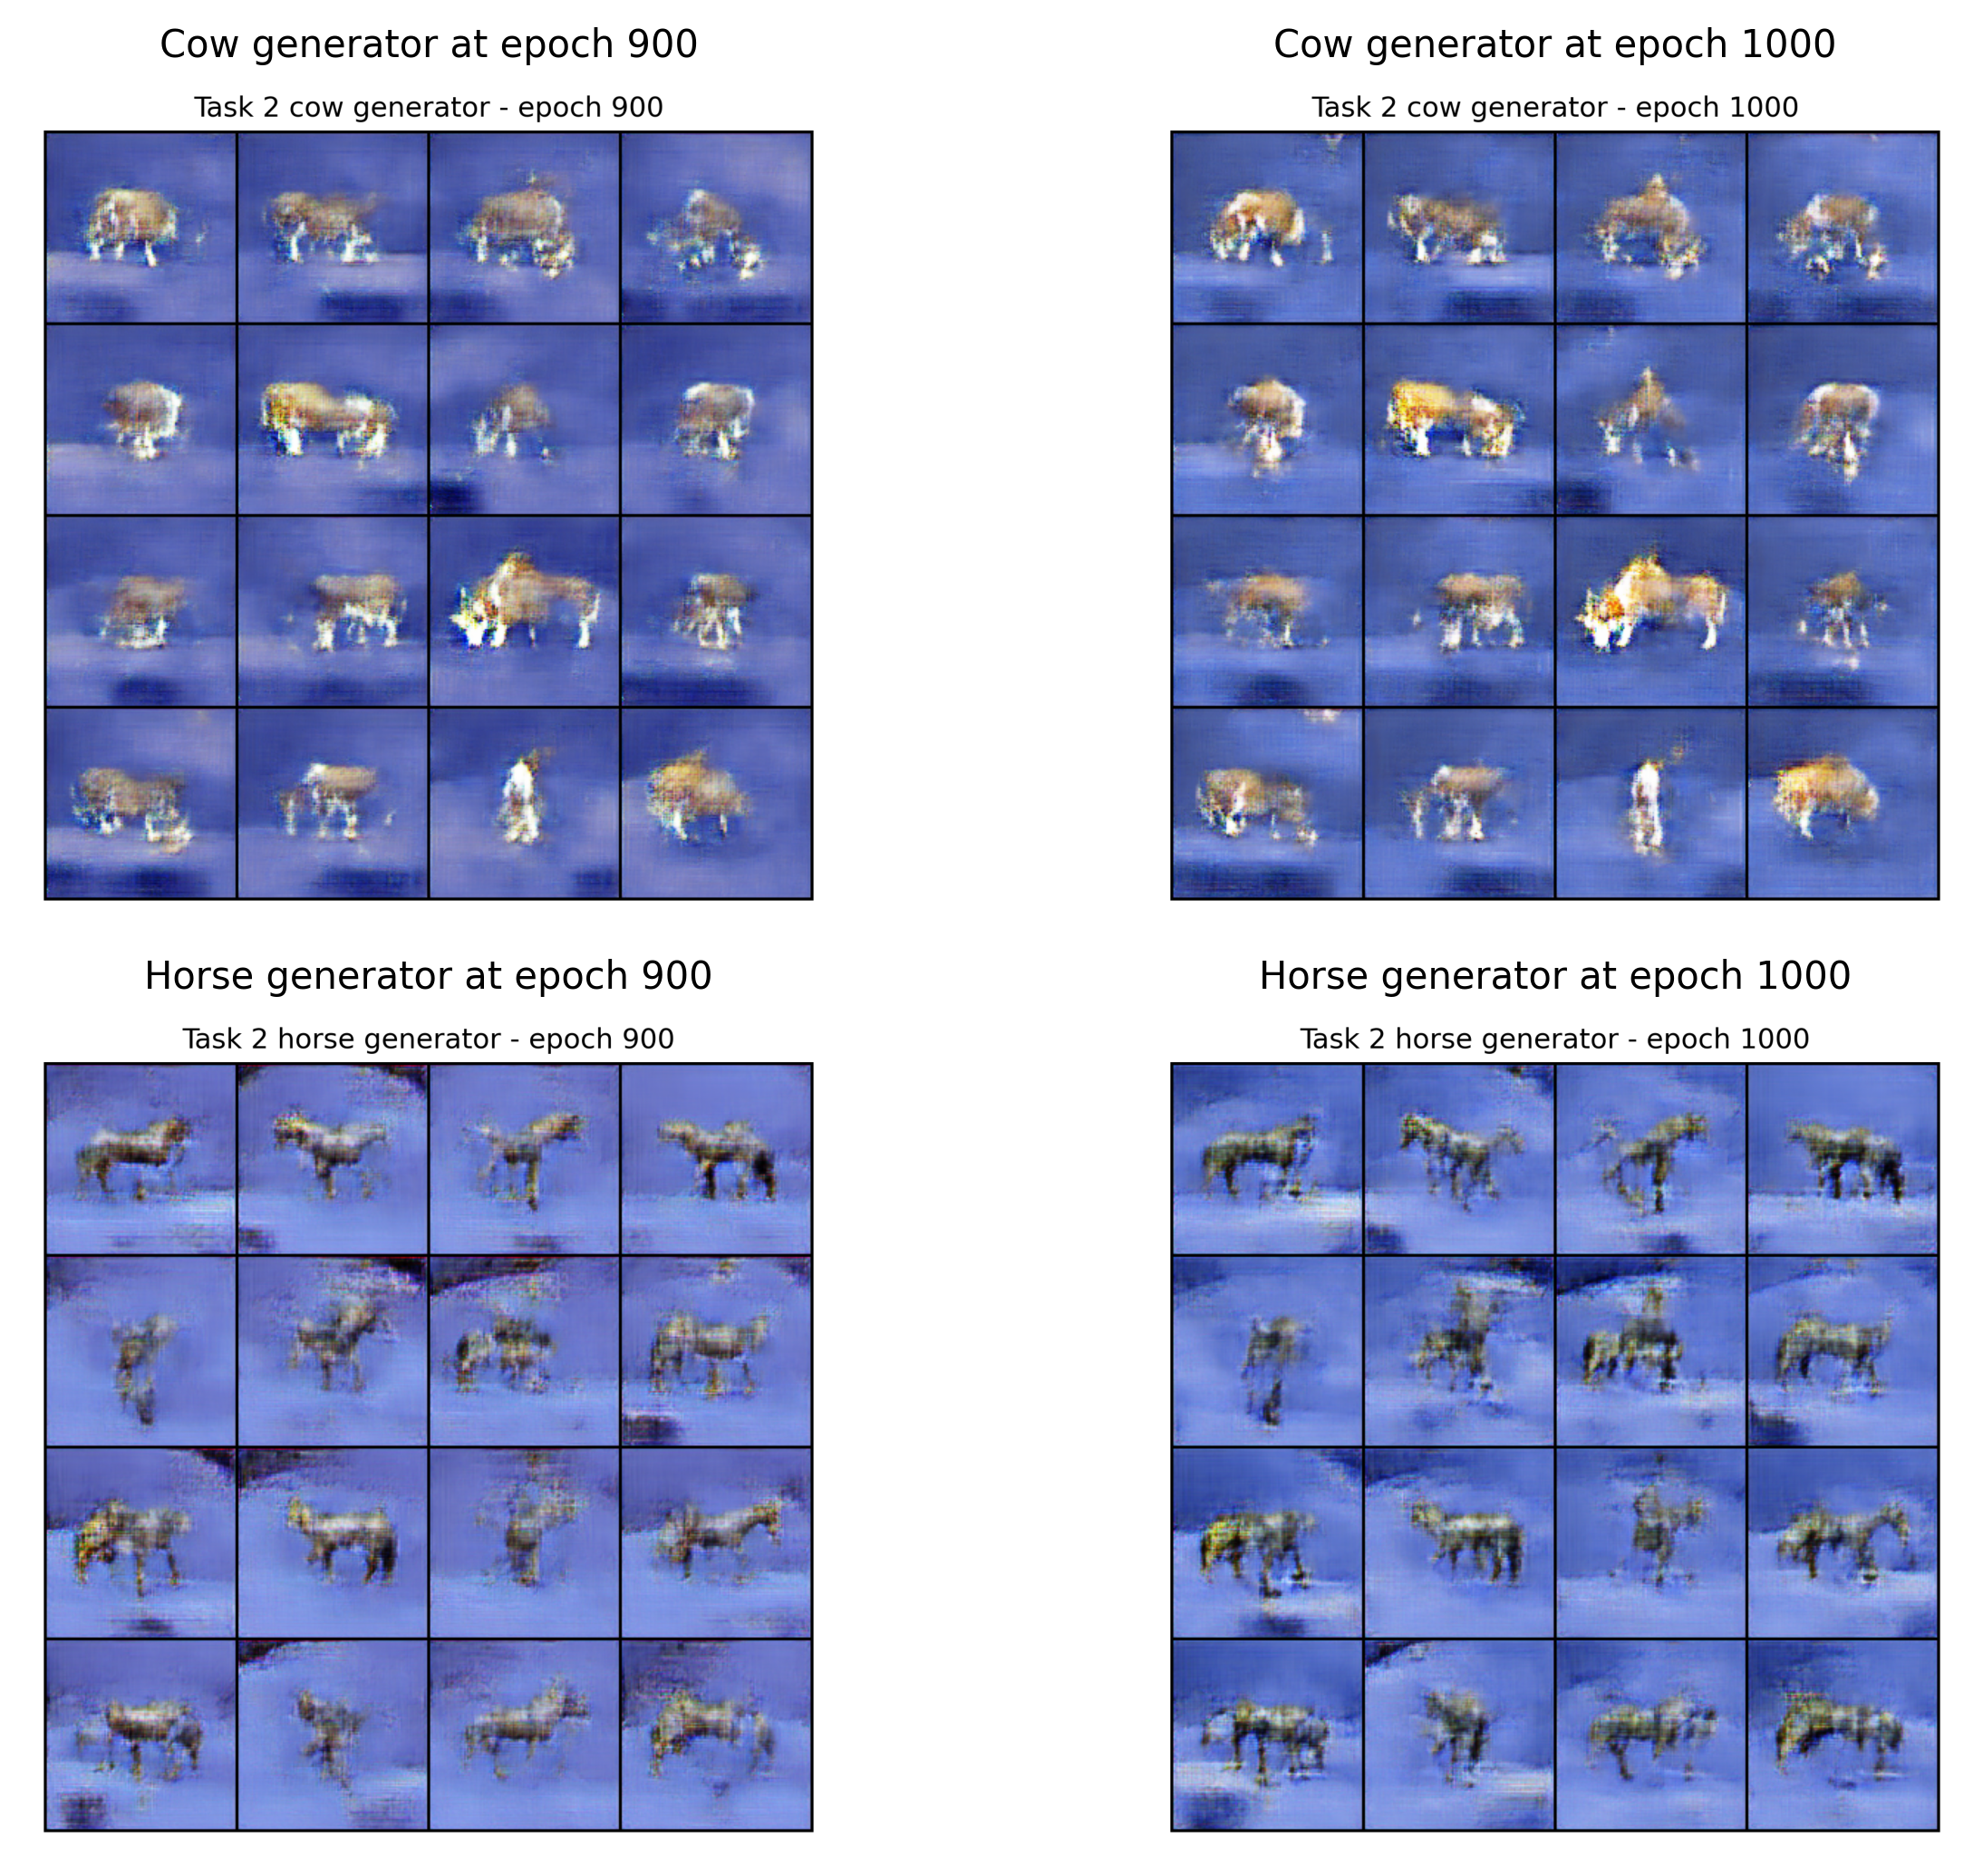
\includegraphics[width=\linewidth,height=0.66\textheight,keepaspectratio]{generated/figures/task2_epoch_grid.png}
\end{columns}
\end{frame}

\begin{frame}{Task 2: Final Augmentation Result}
\footnotesize
\begin{columns}[T]
\column{0.42\textwidth}
\begin{itemize}
  \item Final manual selection
  \begin{itemize}
    \item selected cows = 0
    \item selected horses = 12
  \end{itemize}
  \item Final result
  \begin{itemize}
    \item 65.85\% $\rightarrow$ 67.07\%
    \item cow unchanged
    \item horse: 56.10\% $\rightarrow$ 58.54\%
  \end{itemize}
  \item Key point
  \begin{itemize}
    \item targeted asymmetric augmentation of the weak horse class
  \end{itemize}
  \item Pretrained discriminator
  \begin{itemize}
    \item rejected because horse generations failed visually
  \end{itemize}
\end{itemize}
\column{0.58\textwidth}
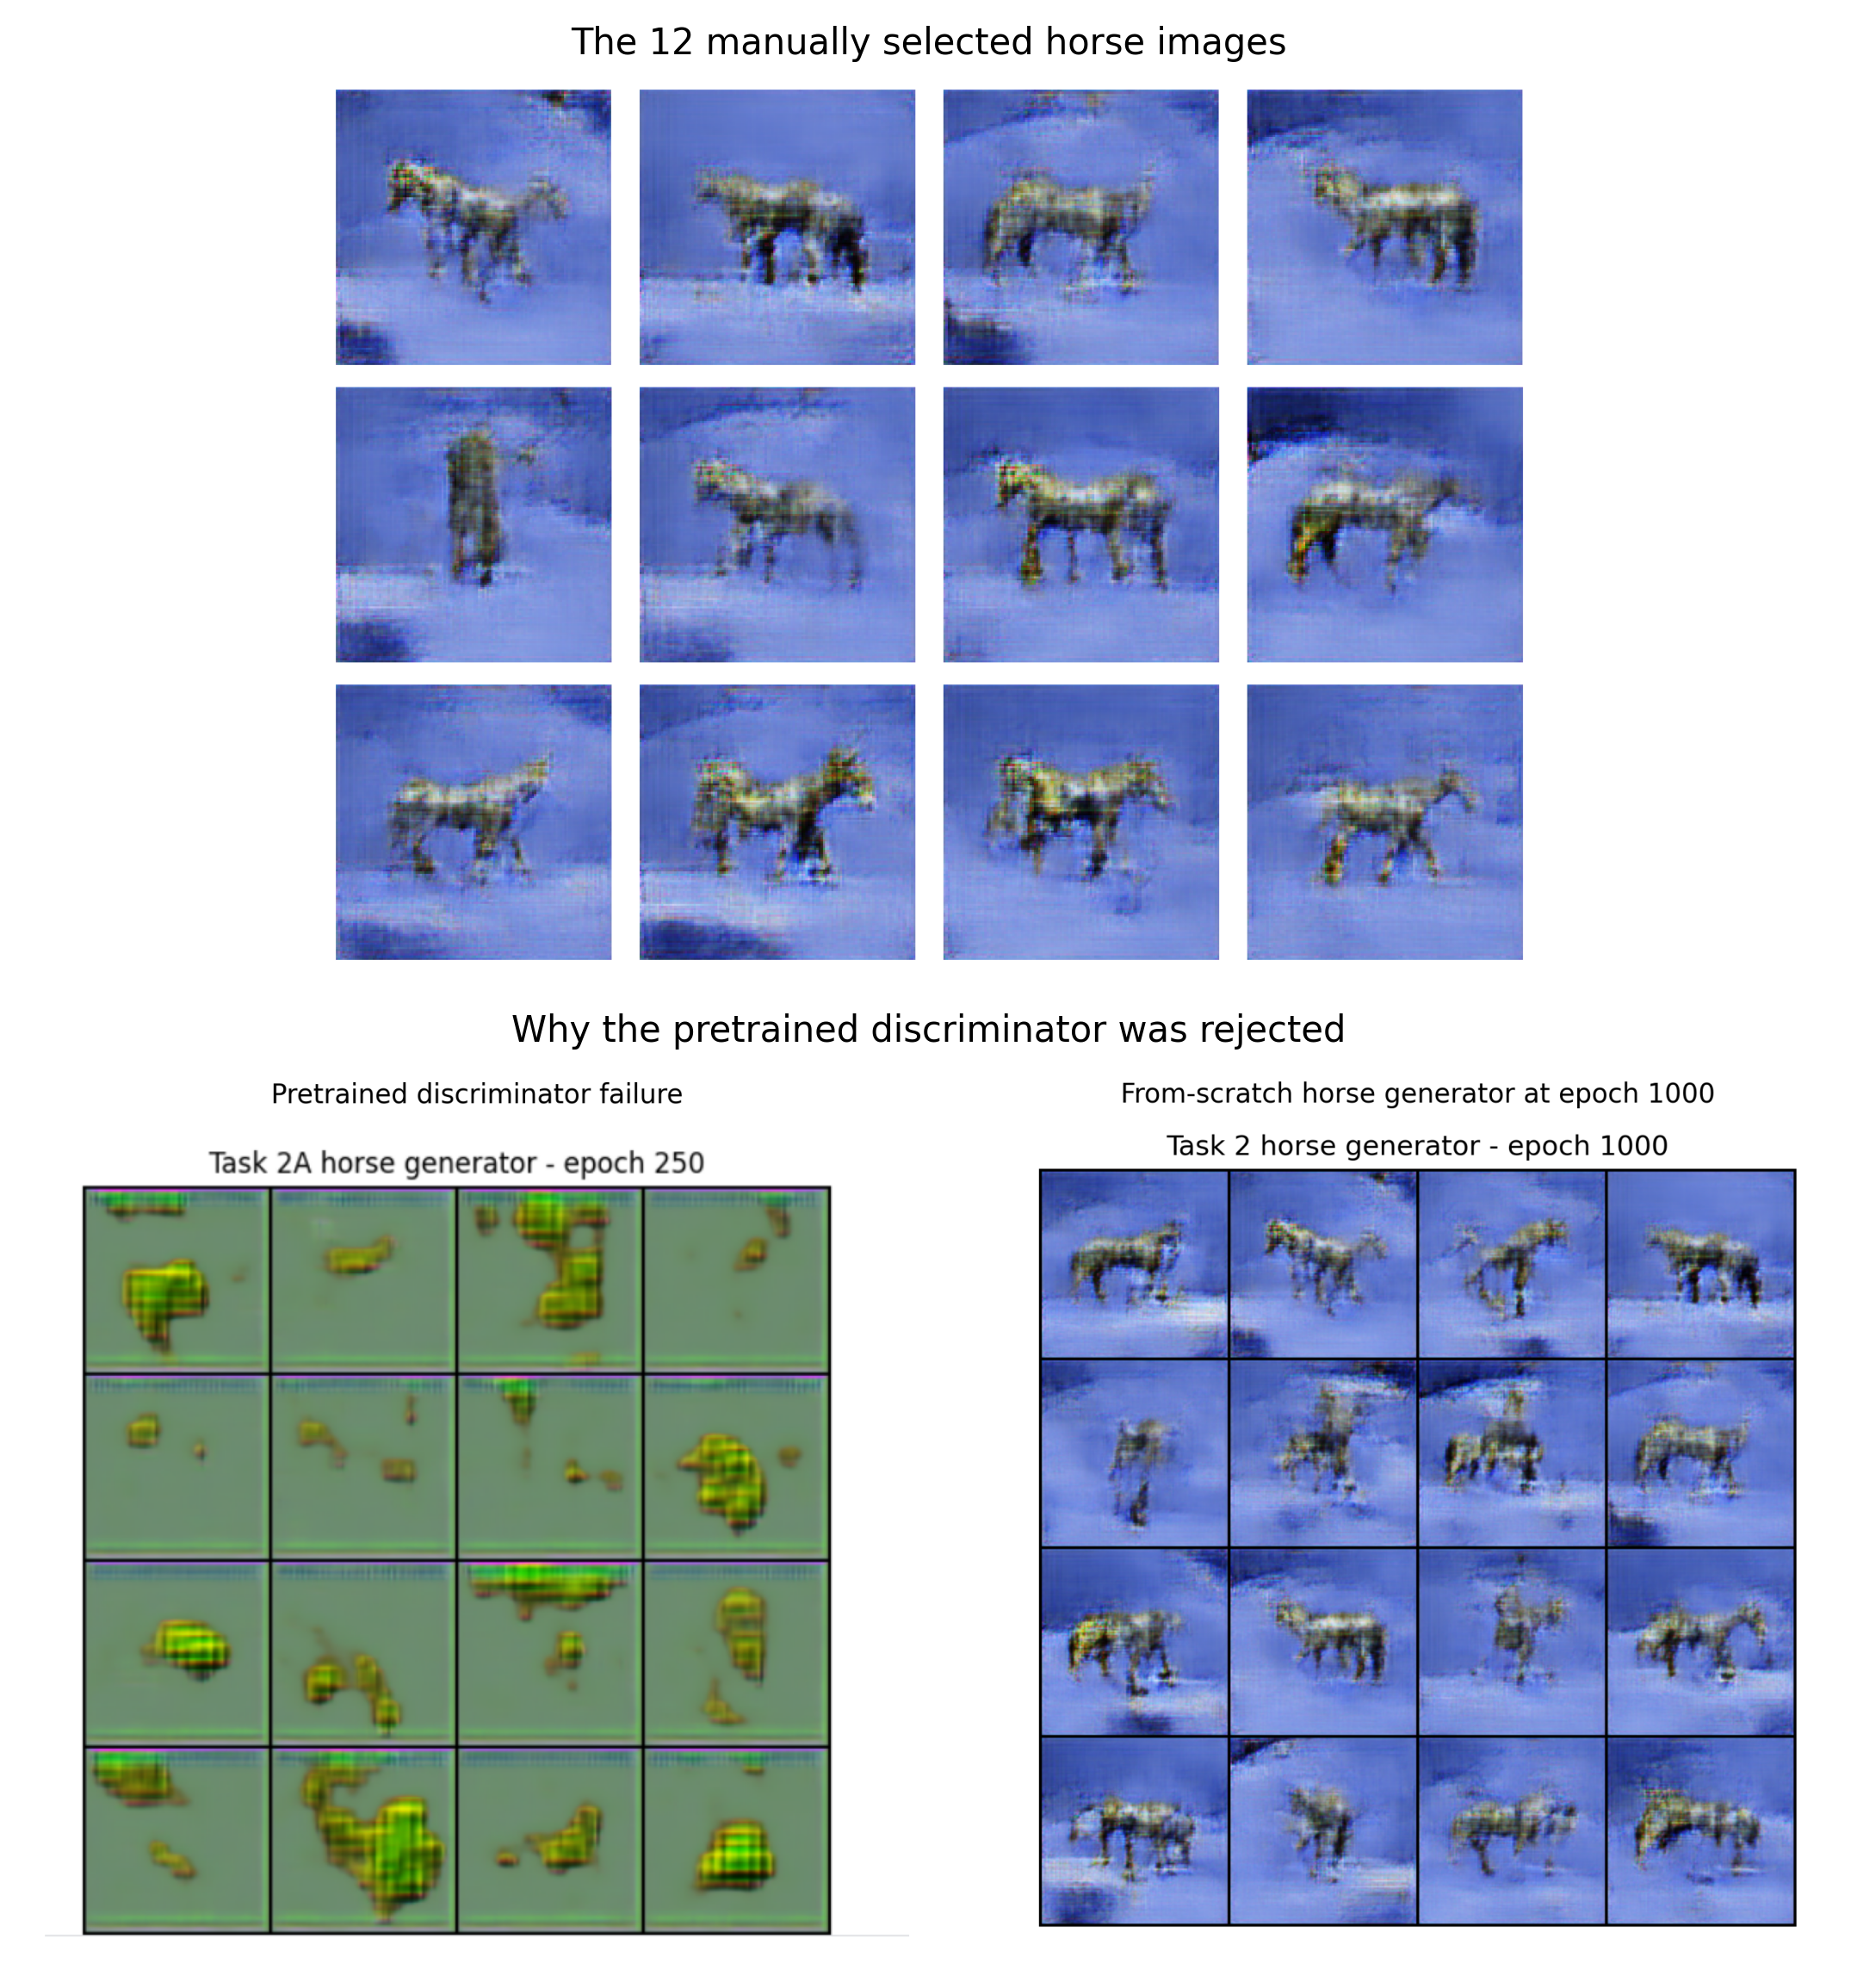
\includegraphics[width=\linewidth,height=0.72\textheight,keepaspectratio]{generated/figures/task2_manual_overview.png}
\end{columns}
\end{frame}

\begin{frame}{Task 3: CycleGAN Design}
\footnotesize
\begin{itemize}
  \item Residual generators
  \begin{itemize}
    \item encoder
    \item residual bottleneck
    \item decoder
  \end{itemize}
  \item PatchGAN discriminators focus on local realism
  \item Training losses
  \begin{itemize}
    \item adversarial loss
    \item cycle-consistency loss
    \item identity loss
  \end{itemize}
  \item Replay buffer reduces discriminator oscillation
  \item Goal
  \begin{itemize}
    \item change visual domain while preserving viewpoint and content structure
  \end{itemize}
\end{itemize}
\end{frame}

\begin{frame}{Task 3: Qualitative Result and Key Point}
\footnotesize
\begin{columns}[T]
\column{0.34\textwidth}
\begin{itemize}
  \item The translations are evaluated qualitatively.
  \item Main visual criteria:
  \begin{itemize}
    \item silhouette
    \item viewpoint
  \end{itemize}
  \item Result
  \begin{itemize}
    \item plausible bidirectional translation
    \item meaningful local style changes
  \end{itemize}
  \item Key point
  \begin{itemize}
    \item compact CycleGAN-style model is sufficient for visual transfer
  \end{itemize}
\end{itemize}
\column{0.66\textwidth}
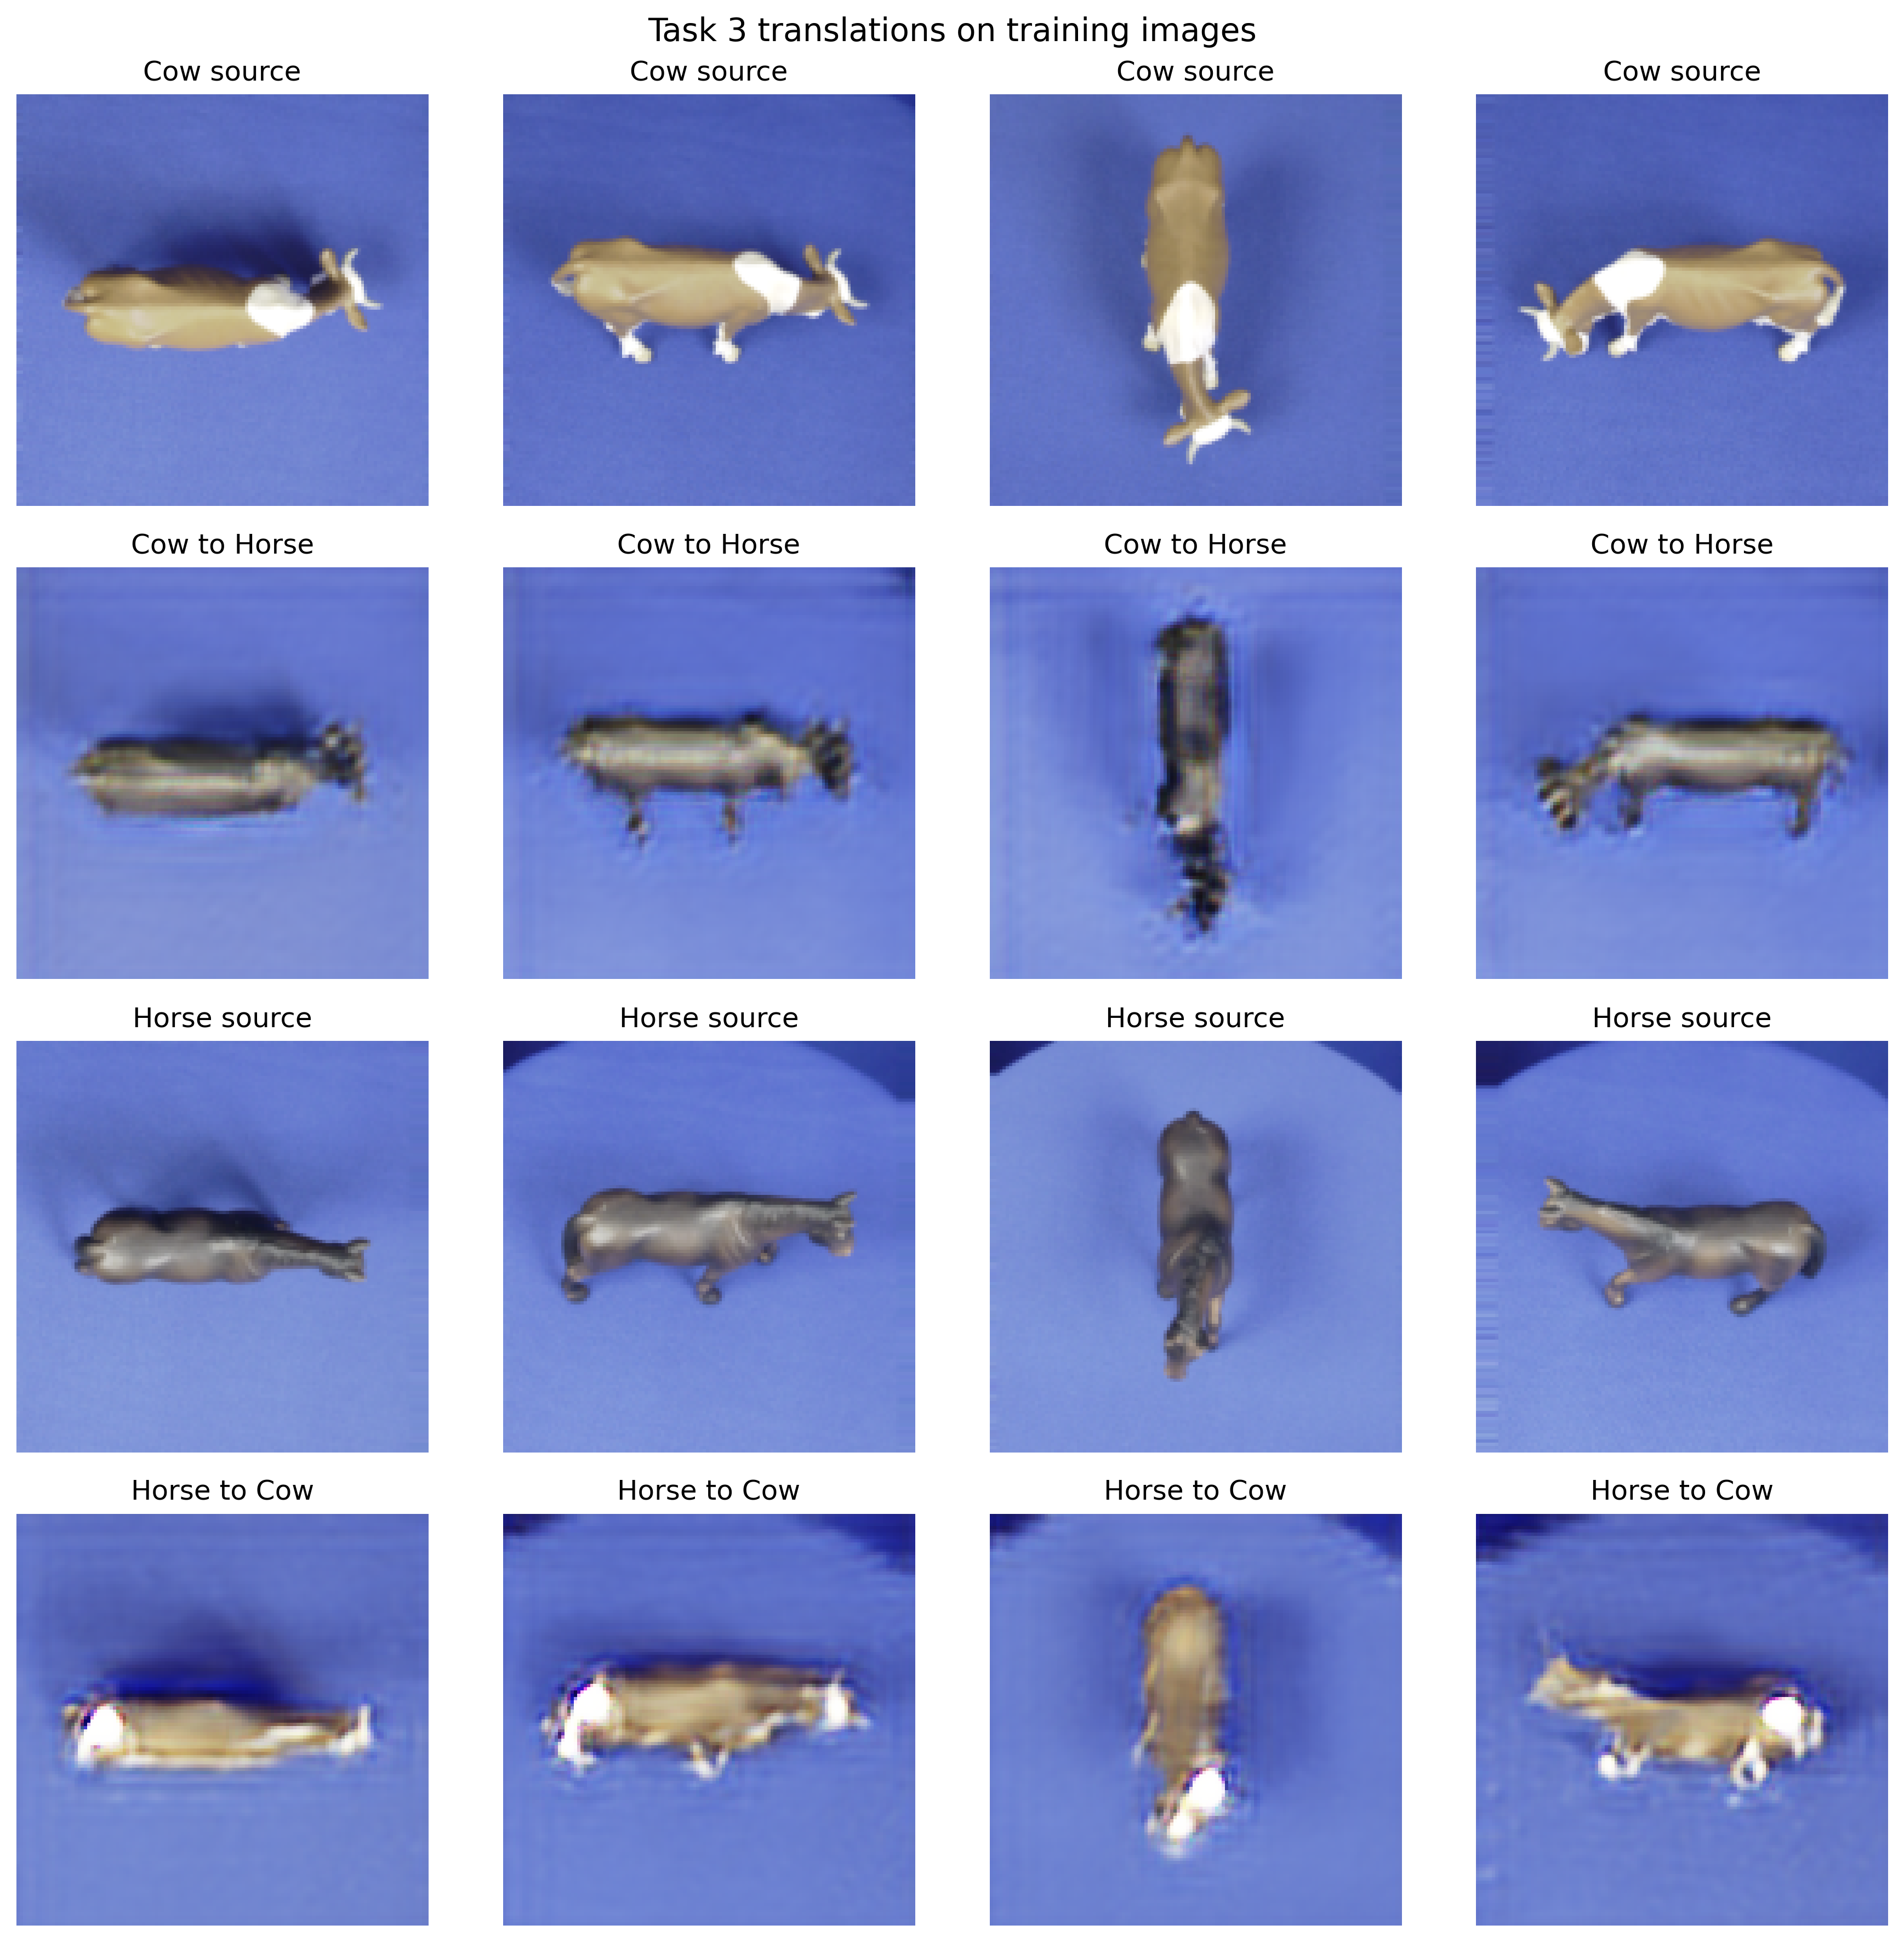
\includegraphics[width=\linewidth,height=0.32\textheight,keepaspectratio]{generated/figures/task3_training_translations.png}

\vspace{0.2em}
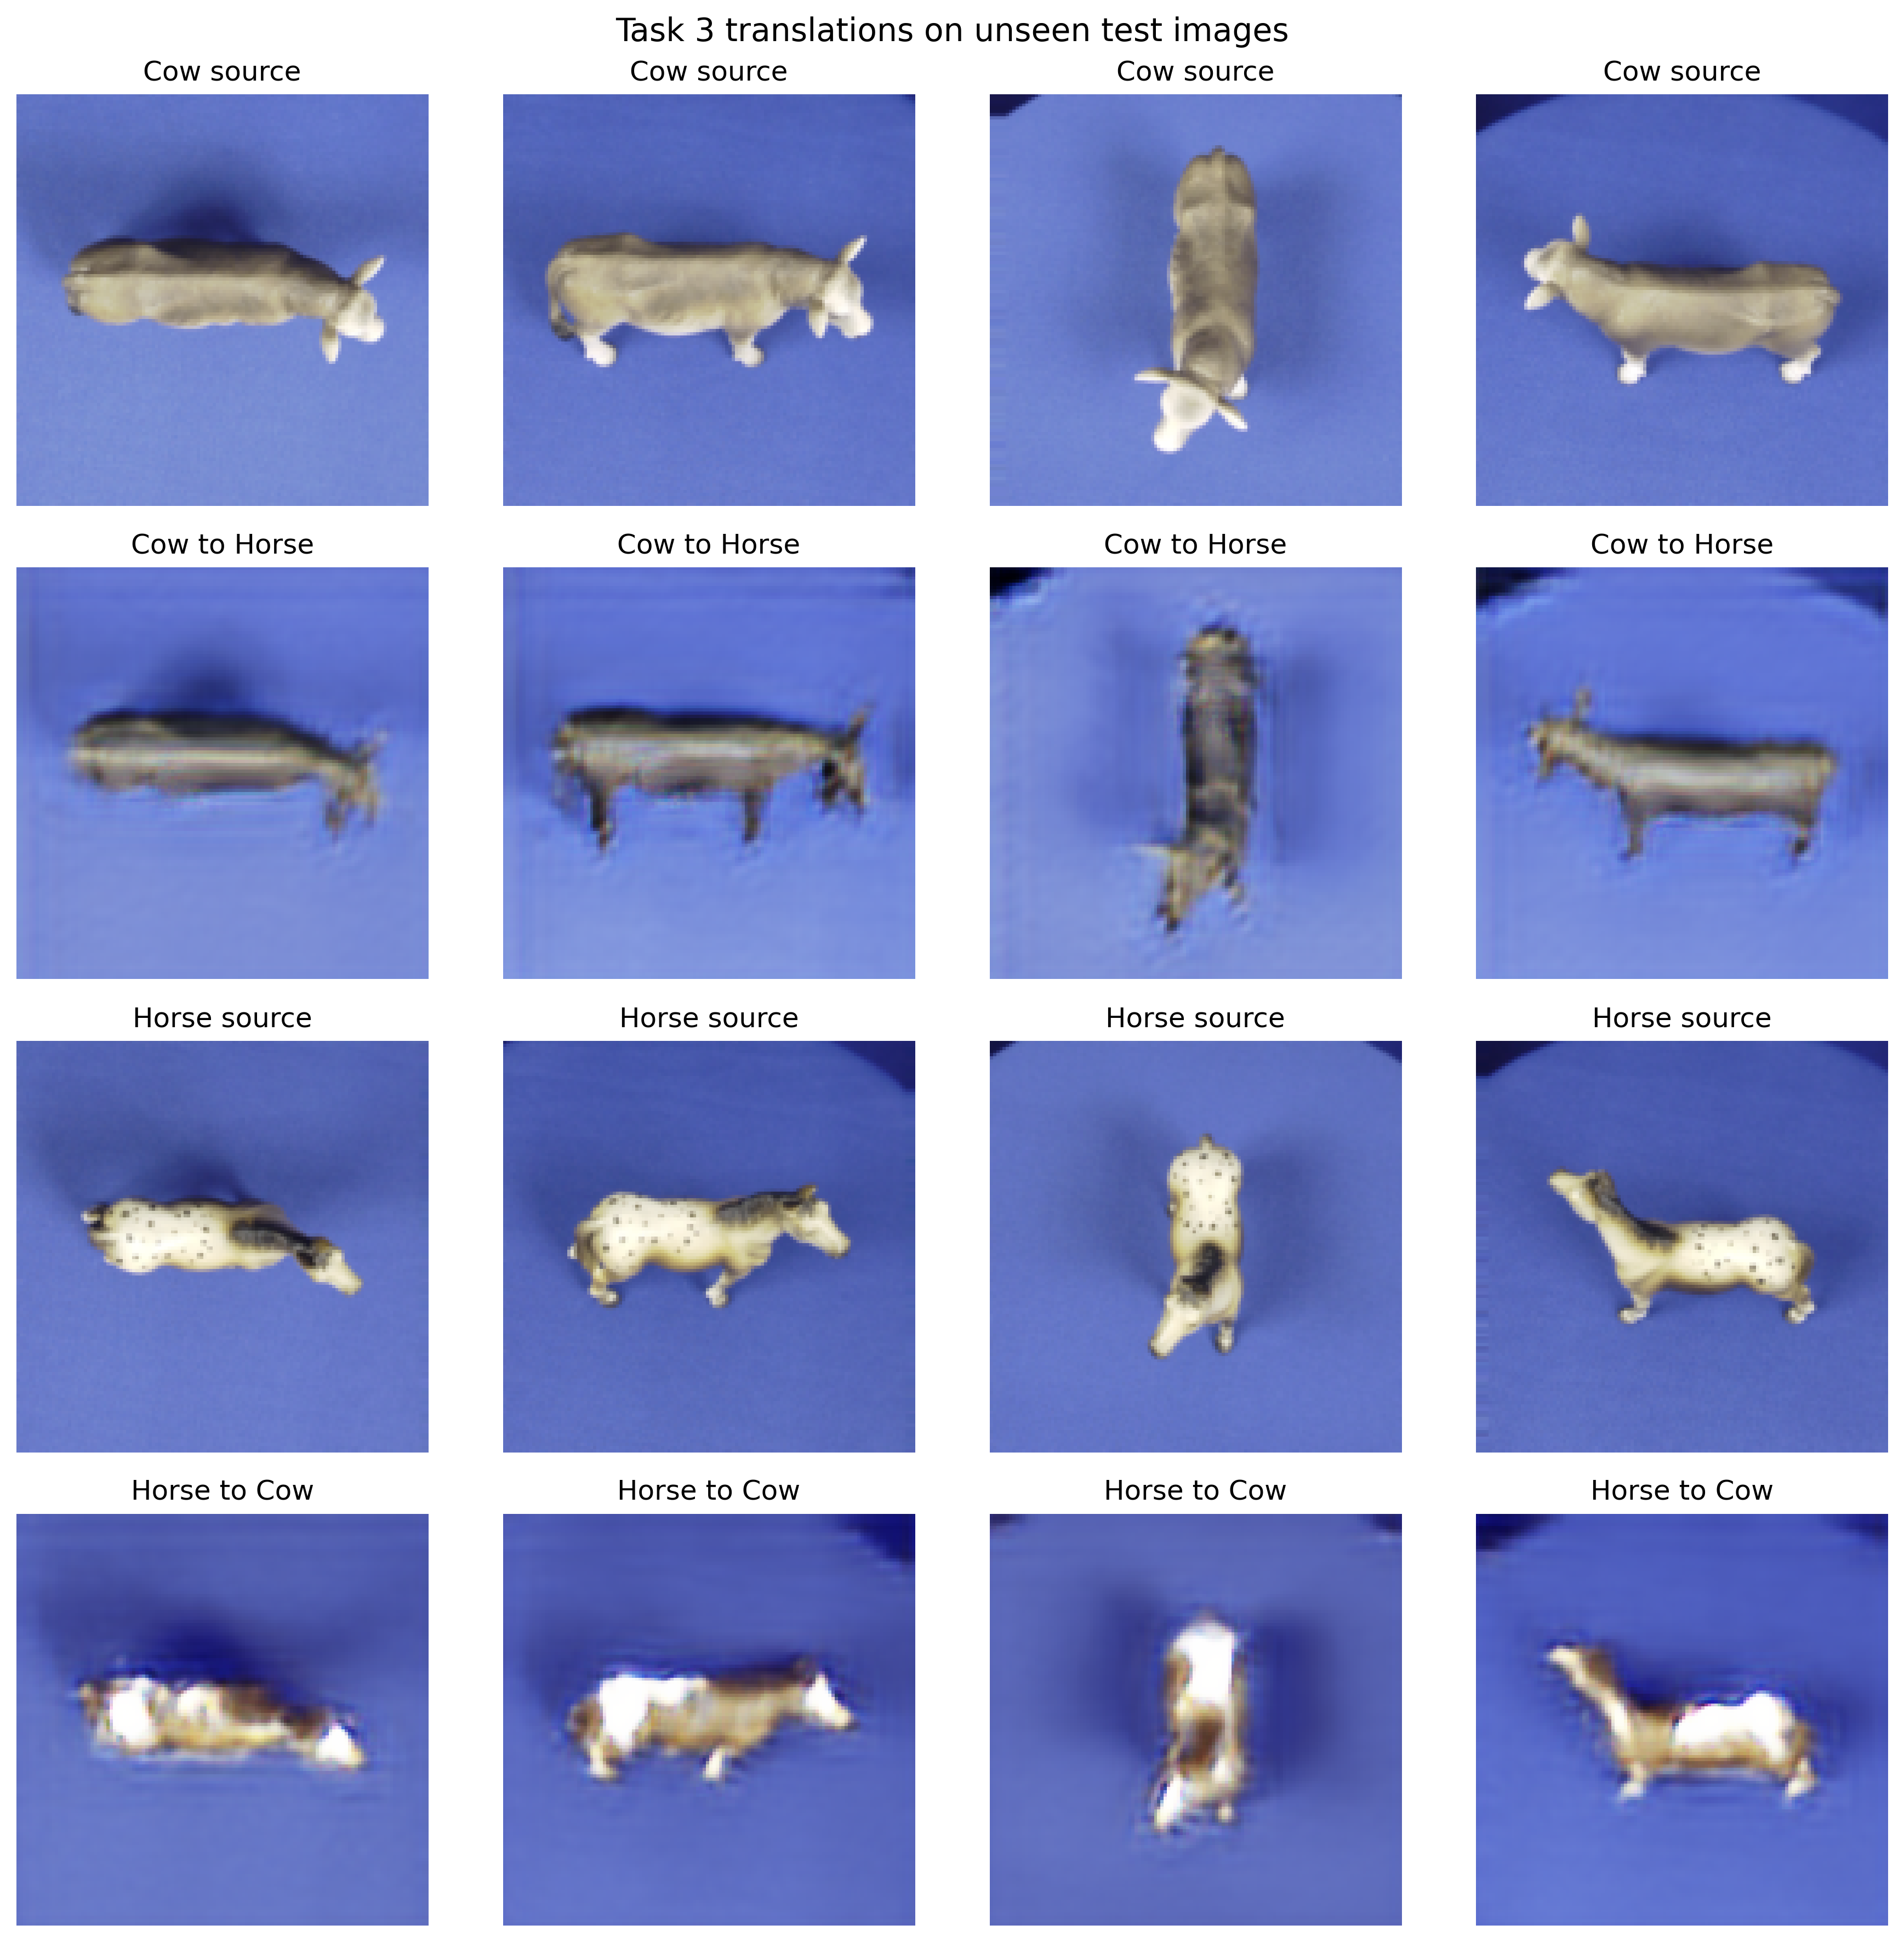
\includegraphics[width=\linewidth,height=0.32\textheight,keepaspectratio]{generated/figures/task3_test_translations.png}
\end{columns}
\end{frame}

\begin{frame}{Conclusion}
\small
\begin{itemize}
  \item A compact from-scratch CNN was sufficient for this dataset.
  \item The key Task 1 choices were:
  \begin{itemize}
    \item class-weighted cross-entropy loss
    \item cow:horse weight ratio = $1:5$
    \item 3-seed logit-level ensemble
  \end{itemize}
  \item Task 2 improved performance only after:
  \begin{itemize}
    \item exporting valid GAN candidates
    \item manually curating the final subset
    \item augmenting the weaker horse class only
  \end{itemize}
  \item Final result:
  \begin{itemize}
    \item Task 1 = 65.85\%
    \item Task 2 = 67.07\%
  \end{itemize}
  \item The best system was not the most complex one.
\end{itemize}
\end{frame}

\end{document}
